In diesem Teil werden alle theoretischen Informationen gegeben, die man für das Verständniss des ganzen Projektes braucht. Nach dieser Einführung sollte man in der Lage sein, den Quellcode im Anhang zu verstehen. Da es jedoch sehr viel Übung erfordert, einen Quellcode zu lesen und zu verstehen, ist es naheliegend, dass der Quellcode nicht verstanden wird. In der Einführung wird grob angeschaut, wie man überhaupt vom Quellcode zur App kommt, im zweiten Teil wird erklährt, wie Daten jeglicher Art als Zahlen in einem Computer abgespeichert werden, im dritten Teil gibt es eine Einführung in die Programmiersprache Java und im letzten Teil werden dann noch ein paar spezifische Informationen in bezug auf Java gegeben, die für die Erstellung einer App gebraucht werden und die Software "`Android Studio"' wird erklährt.

\subsection{Einführung}
\subsubsection{Die IDE}
Die IDE (eng. integrated development environment) oder auf Deutsch die Entwicklungsumgebung ist der Ort, an dem die meisten Programmierer arbeiten. Sie bietet alle wichtigen Werkzeuge, die man zum entwickeln von Software benötigt (Editor mit Color Highlighting, Compiler, Debugger, Dateibrowser etc.). Auf einige Begriffe wird später noch genauer eingegangen. In unserem Falle heisst die Entwicklungsumgebung übrigens Android Studio. In der Entwicklungsumgebung findet die ganze Entwicklung einer Software statt. Der wichtigste Bereich davon ist der Editor. Dort wird der ganze Quellcode hingeschriben und dank Color Highlighting werden die wichtigen Komponenten (Kontrollstrukturen, Variablen, Kommentare etc. siehe Abschnitt 2.3 Grundlagen von Java) mit Farbe hervorgehoben (Abbildung \ref{fig:Colorhighlighting}).
\begin{figure}[htbp] 
  \centering
     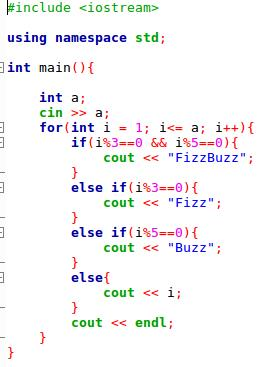
\includegraphics[width=0.3\textwidth]{CodeColor.jpg}
     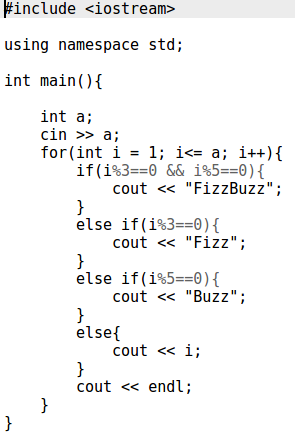
\includegraphics[width=0.3\textwidth]{CodeWithoutColor.png}
  \caption{Beispiel mit und ohne Farbhervorhebung \cite{Colorhighlighting}}
  \label{fig:Colorhighlighting}
\end{figure}
Das ist sehr wichtig, da man ansonsten schnell den Überblick verloren hat. Natürlich gibt es nicht nur eine IDE sondern ganz viele. Welche man davon benutzt ist jedem selbst überlassen. Es gibt auch Entwickler, die es bevorzugen, ohne eine IDE zu arbeiten. Zwar kann man dann alles selbst so gestallten wie es einem passt, es macht aber alles viel komplizierter ist besonders für neu beginnende Programmierer nicht empfehlenswert.

\subsubsection{Der Compiler}
Leider versteht der Computer nichts von dem, was wir in den Quellcode schreiben, alles was er versteht besteht aus Nullen und Einsen (mehr darüber im Abschnitt 2.2). Deshalb muss der für uns verständliche Quellcode in Maschinencode übersetzt werden. Dies geschieht mit dem so gennanten "`Compiler"' (eng. to compile = zusammentragen). Meistens ist dieser bereits in der IDE enthalten und auf Knopfdruck abrufbar. 

\subsubsection{Der Debugger}
Der Debugger ist sehr eng mit dem Compiler verbunden. Meistens schafft man es nähmlich nicht, auf Anhieb einen Fehlerlosen Code zu schreiben. Es passiert extrem schnell, dass irgendwo ein "`;"' oder eine Kontrollstruktur falsch geschrieben wurde (mehr dazu im Abschnitt 2.3). Deshalb ist es sehr wichtig, dass man den Fehler findet. Wenn man jetzt aber Quellcode von 500 Zeilen geschrieben hat, wäre es doch sehr mühsam, wenn man nur wüsste, dass man einen Fehler hat. Genau dafür ist der Debugger. Ist aus dem englischen Wort "`Bug"' entstanden, was so viel wie Käfer heisst, im Programmieren aber als Synonym zu Fehler verwendet wird. Dementprechend könnte man also Debugger als "`Entfehlerer"' oder verdeutscht als "`Fehlersuchprogramm"' bezeichnen. Meistens wird er aber einfach Debugger gennant. Offenbar ist der Debugger dazu in der Lage, die Programmierfehler zu finden. Er findet aber leider nur Syntaxfehler und keine, die den gewünschten Programmoutput betreffen. Man kann sich das so vorstellen: In Microsoft Word werden auch Rechtschreibefehler angezeigt, trotzdem kann man Sätze bilden die entweder keinen Sinn ergeben oder etwas anderes Aussagen, als gewünscht. Aber der Programmieraltag ohne Debugger wäre fast unvorstellbar, da man die meisten Fehler nicht so einfach sieht wie ein falsch geschriebenes Wort. Es gibt verschiedene Arten von Debugger. Die meisten zeigen einem die Fehler erst an, wenn man den Quellcode zu komplieren versucht, es gibt aber auch solche, die das in Echtzeit machen, so wie Microsoft Word Rechtschreibefehler anzeigt. 

\subsubsection{Die Programmiersprache}
Eine Programmiersprache kann man sich am einfachsten wie eine richtige Sprache vorstellen. Sie bildet den Grundbaustein des Programmierens. Bevor man dem Computer etwas  beibringen kann, muss man eine solche lernen. Jede Programmiersprache hat seine eigene Syntax, trotzdem sind sie meistens ähnlich aufgebaut. Sobald man also eine Programmiersprache gelernt hat, fällt es einem einfach, eine nächste zu lernen. Man muss sich das so vorstellen: Nachdem man gelernt hat, wie Windows XP funktioniert, hat man nicht mehr so grosse Schwierigkeiten, zu lernen wie Windows 7 oder Windows 8 funktioniert. Meistens haben die Programmiersprachen verschiedene Anwendungsbereiche: Wird z. B. JavaScript und PHP meist nur in Webanwendungen verwendet, wird C++ wegen seiner Geschwindigkeit meist in Systemanwendungen gebraucht oder Java für Geräte wie Drucker oder eben Androidapplikationen, ausserdem ist das berühmte Computerspiel "`Minecraft"' in Java geschrieben.
\subsection{Vom Binärcode zum Bild}
In diesem Teil geht es darum zu verstehen, wie ein Computer komplexe Informationen wie Bilder speichern kann. Dazu geht man zuerst von Binärcode (z.B. 01110110101001) aus und arbeitet sich dann hoch. Zwar ist dieses Thema nicht unbedingt notwendig, um unser Projekt nachvollziehen zu können, aber es hilft dabei, sich die Datenspeicherung besser vorstellen zu können, was auf jeden Fall sinnvoll ist, da ja die Datenspeicherung eines unserer Kernthemen ist. Ausserdem kann man dann auch die Datentypen in Java besser verstehen (Abschnitt 2.3).
\subsubsection{Vom Binärcode zur Zahl}
Die kleinste Speichereinheit eines Computers ist das Bit. Man sollte das Bit aber auf keinen Fall mit dem Byte verwechseln. Das Byte beinhalted nämlich acht Bits und ist dadurch viel grösser als das Bit. Man kann sich das Bit als Schalter vorstellen: Entweder ist er an oder er ist aus. Es gibt genau diese 2 Zustände. Mit der 1 bezeichnet man den angeschalteten Zustand und mit 0 den ausgeschalteten. Wenn man jetzt zwei Schalter nimmt dann gibt es bereits 4 verschiedene Schalterzustände: 00, 01, 10 und 11. Wenn wir nun $N$ Schalter anneinander reihen haben wir dementsprechend dann auch $2^N$ verschiedene Schalterzustände. Wenn wir jetzt jeden dieser Schalterzustände einer Zahl zuordnen, kann man je nach Schalteranzahl beliebig grosse Zahlen abspeichern. Jedoch wurden Zahlen nicht willkürich irgendeiner Schalterkombination zugeordnet sondern es gibt ein gewisses System dahinter, damit man die Zahlen nachher auch miteinander verrechnet werden können. Dieses System nenn man das binäre Zahlensystem. Es ist nicht wie unser dezimales Zahlensystem auf zehn ausgerichted sondern auf zwei. Um die Zahlen schreiben können, muss aber zuerst deffiniert werden, wie viele Bits gross eine Zahl ist. Diese Definition wird hier der Einfachheit halber auf 4 Bits gesetzt. Wie auch in unserem Zahlensystem wird die Zahl 0 als 0 dargestellt. Weil aber 4 Bits zur Verfügung stehen und nicht nur eines, müssen wir auch den anderen 3 einen Zustand geben, also auch 0. Dann sieh die Zahl 0 also binär dargestellt so aus: 0000. Auch die Zahl 1 ist noch eifach darzustellen: 0001. Wenn aber die Zahl 2 geschrieben werden soll, wird es bisschen komplizierter. Wir können nämlich den ersten Schalter nicht auf auf 2 Stellen. Die Antwort ist aber eigentlich ganz einfach: Wie in unserem dezimalen Zahlensystem nach der Zahl 9 eine neue Stelle gebraucht wird, so wird es binär genau gleich nach der Zahl 1 gemacht. Deshalb wird die Zahl 2 also so geschrieben: 0010. In diesem System geht es weiter: \\
\\
\begin{tabular}{l|l|l|l|l|l|l|l|l|l|l}
Dezimal & 0 & 1 & 2 & 3 & 4 & 5 & 6 & 7 & 8 &  ...\\ \hline
Binär & 0000 & 0001 & 0010 & 0011 & 0100 & 0101 & 0110 & 0111 & 1000 & ...\\
\end{tabular}  \\
\\
Dieses System gut zu kennen kann sehr nützlich sein. Wenn man die Zahlen nämlich noch ein bischen genauer analyziert, kann man feststellen, dass man die hinterste Stelle der binären Zahl immer angibt, ob der Zahl eine 1 addiert werden muss, die zweit hinterste dasselbe mit 2, der dritt hintersten mit 4. Bei jeder weiteren Stelle nach vorne nimmt die dazuzuaddierende Zahl um den Faktor 2 zu. Wenn man dieses System erkannt hat, kann man auch grosse binäre Zahlen in einer nützlichen Frist in eine dezimale übersetzten und umgekehrt. Hier ein Beispiel mit der achtstelligen Binärzahl 10100101:
\\
\begin{tabular}{l l l l l l l l l l l l l l l l l}
$1$ & & $0$ & &  $1$ & & $0$ & & $0$ & & $1$ & & $0$ & & $1$ & & \\
$ 128 $ &+& $0$ &+& $ 32$ &+& $0$ &+& $0$ &+& $ 4$ &+& $0$ &+& $1$ &=& $165$ \\ 
\end{tabular} \\
\\
Das hier vorgestellte binäre Zahlensystem ist jedoch stark vereinfacht, da sich in diesem nur Zahlen $\in \mathbb{N} $ darstellen lassen. Negative Zahlen und Gleitkommazahlen würden aber zu stark vom eigentlichen Thema abweichen. Wichtig ist nur, dass der Computer nur so gennante Maschienenzahlen abspeichern kann. Das heist die Zahlen müssen endlich gross sein und deshalb können periodische und irrationale Zahlen nicht genau abgespeichert werden.
\subsubsection{Grundoperatoren bei binären Zahlen}
Wenn man erst mal verstanden hat, wie das binäre Zahlensystem funktioniert, dann sind die Grundoperationen sehr einfach. Sie lassen ganz einfach mit den schriftlichen Operationen berechnen. Als Beispiel werden 5 Bit grosse Zahlen genommen: Die Zahl 6 (00110) und die Zahl 3(00011).
\paragraph{Addition}
\begin{tabular}{llllll}
&0&0&1&1&0 \\
+&0&0&0&1&1 \\ \hline
&0&1&0&0&1
\end{tabular}
\paragraph{Subtraktion}
\begin{tabular}{llllll}
&0&0&1&1&0 \\
-&0&0&0&1&1 \\ \hline
&0&0&0&1&1
\end{tabular}
\paragraph{Multiplikation}
\begin{tabular}{lllllllllll}
0&0&1&1&0& $\cdot$ &0&0&0&1&1 \\ \hline
&&&&&&0&1&1&0&0 \\
&&&&&&0&0&1&1&0 \\ \hline
&&&&&&1&0&0&1&0
\end{tabular}
\paragraph{Division}
\begin{tabular}{lllllllllll l}
0&0&1&1&0& : &0&0&0&1&1 & = 0 0 0 1 0 \\ \hline
 & &1&1& & &&&&&& \\ \cline{3-4}
 & &0&0&0& &&&&&& \\ 
\end{tabular}
\subsubsection{Von der Zahl zur Text}
Mit dem Wissen, wie Zahlen binär gespeichert werden, kann man dann sehr eifach verstehen, wie Texte abgespeichert werden. Im Grundsatz ist es nur eine willkürliche Zuordnung von Zeichen zu einer Zahl. Es gibt verschiedene Zuordnungen, die wichtigsten hierbei sind ASCII (American Standart Code for Information Interchange) und UTF-8(Universal Character Set Transformation Format). ASCII hierbei speichert jegliche Zeichen in 7 Bits ab und kann aber nur 128 verschiedene Zeichen speichern. Zum Beispiel würde man das Wort Haus so kodieren: 72 97 117 115. Wenn man diese Zahlen auch noch in Bits übersetzt, hat man die exakte Kodierung, wie sie auch auf dem Computer abgespeichert würde: 1001000110000111101011110011(siehe Abbildung \ref{fig:ASCII})
\begin{figure}[htbp] 
  \centering
     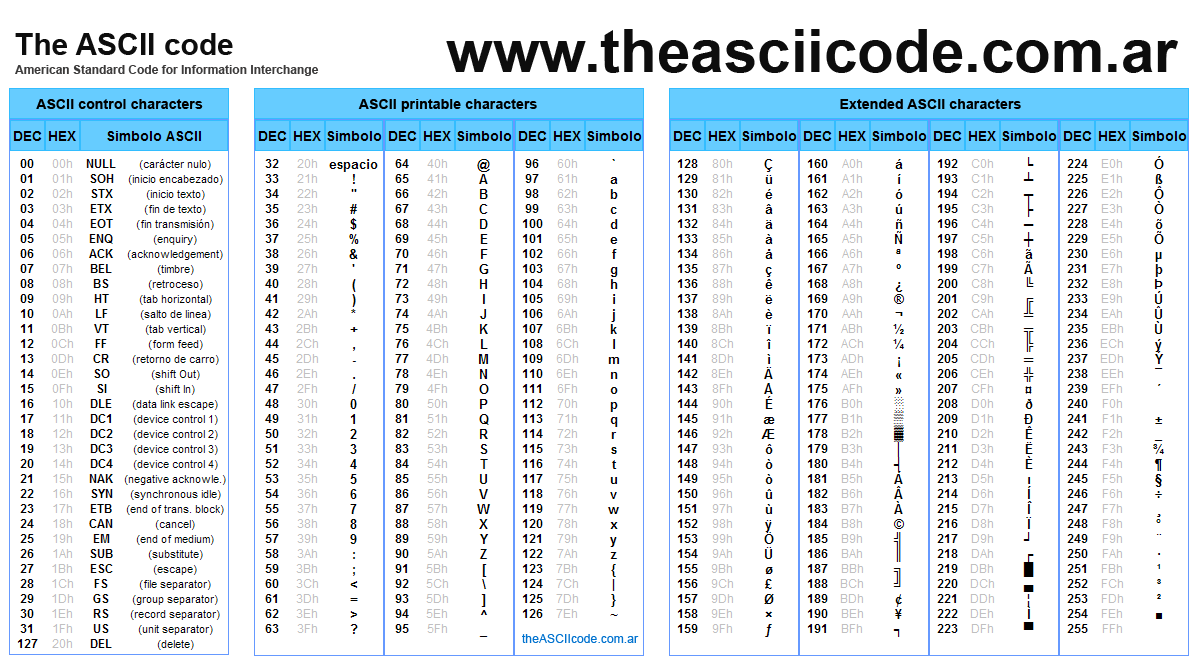
\includegraphics[width=1\textwidth]{ASCII.png}
  \caption{ASCII Tabelle \cite{ASCII}}
  \label{fig:ASCII}
\end{figure}
Dadruch werden viele sprachspezifischen Zeichen wie die deutschen Umlaute nicht abspeicherbar. Deshalb wird ASCII heutzutage auch meistens nicht mehr gebraucht. UTF-8 ist hierbei viel nützlicher, aber auch komplizierter. Es kann jegliche Spezialzeichen jeder Sprache abspeichern. UTF speichert die einfachen ASCII Zeichen in 8 Bits ab, das erst hinzugekommene Bit speichert ab, ob es sich bei dem Zeichen um ein ASCII Zeichen handelt oder nicht. Falls ja, können die restlichen sieben Bits wie ein ASCII Zeichen interpretiert werden. Ansonsten folgen nicht nur 7 Bits sondern wieder abhängig von der nächsten Zeichenfolge bis zu 31 weitere Bits (im ganzen dann 4 Bytes). Die deutschen Umlaute brauchen zum Beispiel 2 Bytes Speicherplatz. UTF-8 ist heutzutage der meist verbreitete Zeichensatz im Internet (im November 2016 benutzen rund 88\% aller Webseiten UTF-8). \cite{UTF-8} Ein weiterer heutezutage sehr verbreiteter Zeichensatz ist Unicode, auf diesen wird hier aber nicht weiter eingegangen.
\subsubsection{Von der Zahl zur Farbe}
Um Bilder abspeichern zu können, muss man zuerst einmal wissen, wie Farben abgespeichert werden. Die meist verbreitete Methode für das Abspeichern von Farben ist RGB (eng. Red Green Blue). Der Name spricht für sich, nacheinander wird die Menge der Farbe Rot, Grün und Blau in einer Skala von 0 bis 255 angegeben. Aber auch die Farben werden in einem unüblichen Zahlensystem dargestellt: im Hexadezimalen. Dieses basiert nicht wie das binäre auf 2 und das dezimale auf 10, sondern auf 16. Da in unserem Zahlensystem keine Ziffer für 10-15 existieren, hat man dier ersten Buchstaben des Alphabetes genommen. 10 wäre also "`A"' und 15 wäre "`F"' hexadezimal geschrieben. \textbf{Achtung: Wegen diesem System ist die hexadezimale 10 nicht dasselbe wir die dezimale 10 sondern 16.} 255 wäre dementsprechend "`FF"' hexadezimal geschrieben und somit die grösste hexadezimale Zahl, die mit zwei Ziffern geschrieben werden kann. Das ist natürlich kein Zufall sondern extra so gewählt. Um eine hexadezimale Zahl zu kennzeichnen, benutzt man in der Regel den Präfix 0x. Ein RGB wert besteht also aus drei zwei stelligen hexadezimalen Zahlen. Meistens wird bei RGB-Farben ein \# als Präfix verwendet anstatt des hexadezimal üblichen 0x. Auch noch wichtig anzumerken ist, dass das RGB-System ein additiver Farbraum ist. Das heisst also wenn man die volle Farbstärke aller Farben Rot, Grün und Blau verwendet, erhält man weiss. Hier nun eine Tabelle mit den wichtigsten Farben und dem dazugehörigen hexadezimalen Wert. \\
\\
\begin{tabular}{|l|l|l|l|}
\hline
Rot & Grün & Blau & Weiss \\ \hline
\#FF0000  & \#00FF00 & \#0000FF & \#FFFFFF \\ \hline
Schwarz & Gelb & Magenta & Cyan \\ \hline
\#000000 & \#FFFF00 & \#FF00FF & \#00FFFF \\ \hline
\end{tabular} \\
\\
Übrigens ist es auch kein Zufall, dass die Farben hexadezimal dargestellt werden und nicht dezimal. Ein System, welches auf zehn basieren würde, hätte immer ein gewissen Datenverlust, da man um 10 darstellen zu können 4 Bits braucht. Mit 4 Bits lassen sich aber Zahlen bis 16 darstellen. Um also mit demselben Speicherbedarf die maximale Speicherausnutzung zu erreichen, hat man sich für ein hexadezimales System entschieden. Es gibt auch hier nicht nur ein System, ein weiteres sehr wichtiges Farbsystem ist das "`CMYK"', welches vor allem für Drücker verwendet wird. Dieses System ist im Gegensatz zum RGB-Farbsystem ein subtraktives. Der Name steht für Cyan Magenta Yellow Key. Auch wie im RGB-Farbsystem werden mit Cyan, Magenta und Gelb die Menge der Farben dargestellt. Das CMYK-Farbsystem besitzt aber noch einen vierten Wert: Den Schwarzanteil (hier mit K für Key angegeben um nicht mit B für Black um eine Verwechslungsgefahr mit Blue zu vermeiden).
\subsubsection{Von der Farbe zum Bild}
Nun sollten alle Grundlagen vorhanden sein, um zu verstehen, wie ein Bild gespeichert werden kann. Hier wird zuerst von einem total unkomprimierten Bild ausgegange, das mit RGB Farben ausgestattet ist. Digitale Bilder können in zwei Gruppen unterteilt werden: Rastergrafiken und Vektorgrafiken. Zuerst wir ersteres angeschaut. Ein Computerbildschirm ist bekanntlicherweise aus einzelnen Pixeln aufgebaut. Jedes dieser Pixel funktioniert eigenstädnig und kann eine belibige Farbe anzeigen. Heutzutage ist das wohl am weitesten Verbreitete Bildschirmformat das Full-HD mit 1920x1080 Pixeln. In einem völlig unkomprimierten Bild wird also für jedes Bild seine eigene Farbe gespeichert und schon hat man sein Bild abgespeichert. Wir aber aus dem letzt Kapitel über Farben bekannt ist, werden die Farben üblicherweise mit RGB abgespeichert. Wenn man nun bedenkt, wie diese Zahlen binär aufgebaut werden, kommt man für jede hexadezimale Stelle auf 4 Bits, die gebraucht werden. Weil eine normale RGB-Farbe aus 6 hexadezimalen Zahlen bestehen, heisst das wiederum, dass eine RGB-Farbe mit 24 Bits geschriben werden kann, was das gleiche wie 3 Bytes ist. Um also ein Bild abzuspeichern, werden $1920 \cot 1080 \cdot 3=6220800$ Bytes $ \approx  6.5$ Megabytes. Das ist bereits eine sehr grosse Datenmenge. Für Qualitativ hochwertige Bilder ist die Auflösung aber oftmals grösser und die Farbe genauer, wodurch der Bildspeicherplatzbedarf nochmals enorm wachsen würde. Wenn man jetzt sogar ein Video mit 60 FPS (eng. Frames Per Second = Bilder pro Sekunde) mit dieser Datengrösse des errechnetetn Bildes mit 6.5MB  speichern würde, würde man für jede Sekunde 390MB verbrauchen. Dadurch wäre also ein Film mit einer durschnittlichen Länge von 1.5h 2.106TB gross, also grösser als die meisten Speicher eines Computers. Die Realität sieht aber ganz anders aus: Um Speicherplatz zu optimieren werden erstens bei Bildern komprimierungen angewendet, welche über komplexe Algorithmen die Bilder so abspeichern, dass diese viel weniger Speicherplatz einnehmen. Ausserdem speichern Videos nicht jedes Bild neu sondern nur dessen Veränderung. So kommt man dann auf eine etwa 1000 mal kleinere Speichergrösse. Bei Bildkompression unterscheidet man übrigens auch zwischen verlustbehafteten Kompressionen und verlustfreien. Bekannte verlustfreie Kompressionen sind zum Beispiel TIFF und PNG und bekannte verlustbehaftete JPEG und GIF \cite{Dateiformate}. Jedes Dateiformat hat aber seine eigenen Vorteile und Nachteile und je nach Zweck solle man sich überlegen, welches davon am meisten Sinn macht. Wie Anfangs erwähnt gibt es aber auch noch die Vektorgrafik. Die Vektorgrafik speichert keine Informationen über einzelne Pixel sondern es speichert zum Beispiel eine Linie oder ein Kreis mit einer Funktion. Der Vorteil einer Vektorgrafik ist, dass man diese frei skalieren kann, ohne dass man eine Qualitätseinbusse hat. Meistens sind Firmenlogos und Ähnliches mit einer Vektorgrafik geschrieben.
\subsection{Grundlagen von Java}

\subsection{Android Studio}